\documentclass{livre}

\titre{Patchwork combinatoire de courbes algébriques}
\soustitre{Mémoire de L3}
\auteurs{Raphaël \bsc{Alexandre}, Thomas \bsc{Mordant}}
\externes{Encadré par : \\ Ilia \bsc{Itenberg}}
\lieu{\'Ecole Normale Supérieure}
\date{\today}

\newcommand{\der}[3]{\at{\frac{\partial #1}{\partial #2}}{#3}}


\bibliography{bibliographie}


\begin{document}

\tableofcontents

\newpage
\chapter{Introduction du problème}
Bonjour,
avant le propos central de ce texte, nous allons essayer d'exposer le problème étudié ainsi que de poser les premières notations utilisées.

\section{Le seizième problème de \textsc{Hilbert}}

Le problème est le suivant. \'Etant donné une polynôme homogène $F(x_0,x_1,x_2)$ à coefficients réels et de degré $d$, quelles sont les qualités topologiques de ses zéros dans le plan projectif réel, $\P^{2}(\R)$ ? 

Par la suite, nous supposerons toujours que les zéros de $F$ sont non-singuliers.

Nous désignerons par $\R F$ l'ensemble des zéros de $F$, qui a alors  naturellement une structure de variété lisse. Une variété lisse fermée de dimension $1$ dans un espace compact est une union de cercles. Ainsi, $\R F$ sera une collection de cercles.


\paragraph{Pour $d=1$}Nous observons que \[ F(x_0,x_1,x_2) = ax_0 + bx_1+cx_2 \]avec $a,b,c\in \R$. Ainsi, $\R F$ est une droite de $\R^{2}$. Son plongement dans $\P^{2}(\R)$ est un grand cercle.

\subsection*{Plongements de $\R^{2}$ dans $\P^{2}(\R)$}

Il est utile de garder à l'esprit que deux plongements possibles dans $\P^{2}(\R)$ donnent lieu à un cercle :

\begin{itemize}
\item le plongement d'une droite de $\R^{2}$ (qui donne un grand cercle qui intersecte la droite à l'infini en un point) ;
\item le plongement d'une conique de $\R^{2}$ (que nous appellerons \textit{ovale}).\note{Quelques doutes dessus, il faudrait vérifier si c'est le plongement d'une conique ou d'autre chose ...}
\end{itemize}

Le plongement d'un ovale divise $\P^{2}(\R)$ en deux régions non connectées : une boule et un ruban de \textsc{Möbius}.\note{Est-ce que c'est aussi vrai pour les grands cercles ?}

\subsection*{Classification en petits degrés}

\paragraph{Pour $d=2$}Si nous revenons au problème initial, pour $d=2$ nous avons $F$ qui décrit une conique de $\P^{2}(\R)$, c'est donc ou bien un ovale ou bien l'ensemble vide (ce qui se produit lorsque $F$ est définie).

\lemme{ 
Nous montrerons que :
\begin{itemize}
\item lorsque $d$ est pair, $\R F$ est une réunion d'ovales ;
\item lorsque $d$ est impair, $\R F$ est la réunion d'une droite et d'ovales.
\end{itemize}
}{}

\paragraph{Pour $d=4$}La classification pour $d=4$ nous donne la distinction de cas suivante sur la composition de $\R F$:
\begin{itemize}
\item cela peut être l'ensemble vide ;
\item un, ou deux, ou trois, ou quatre ovales ;
\item un ovale dans un autre tel que dans la figure qui suit.
\end{itemize}

\begin{figure}[H]
\begin{center}
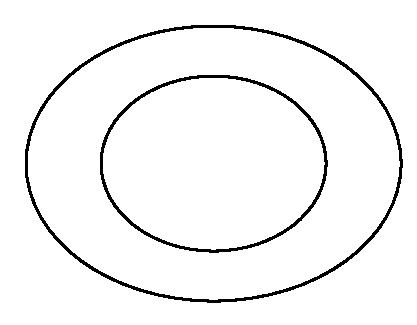
\includegraphics[scale=0.6]{Figures/fig1}
\end{center}
\caption{Lorsque $d=4$, un ovale peut être dans un autre}\label{fig1}
\end{figure}

Mais le cas suivant est impossible :
\begin{figure}[H]
\begin{center}
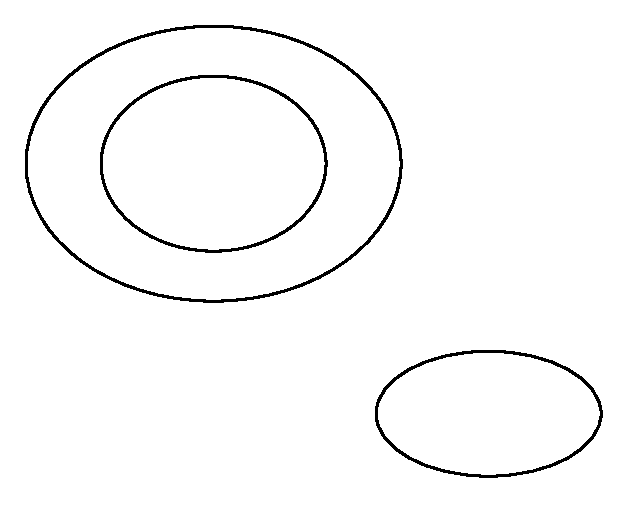
\includegraphics[scale=0.6]{Figures/fig2}
\end{center}
\caption{Ceci est impossible}
\end{figure}
En effet, si nous traçons une droite qui coupe chacun des ovales en deux points, nous obtenons $6$ points d'intersections alors que le degré de l'équation sous-jacente est de $4$.
\begin{figure}[H]
\begin{center}
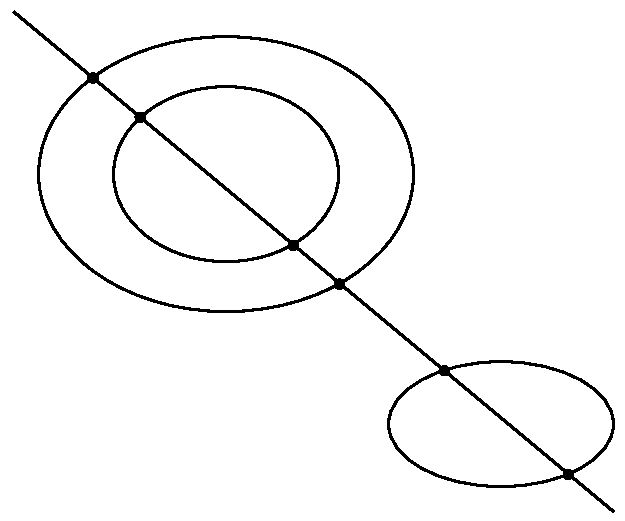
\includegraphics[scale=0.55]{Figures/fig3}
\end{center}
\caption{Les six points d'intersections contredisent $d=4$}
\end{figure}

Nous procédons de même avec le cas où nous aurions $5$ ovales. Par leurs $5$ centres passe une conique et l'intersection est de $10$ points alors qu'il devrait y en avoir au plus $4\times 2 = 8$.\note{Introduction à compléter}

Il est utile de mentionner le résultat suivant qui donne la classification topologique (mais ne donne pas de classification sur le plongement).
\lemme{ 
Soit $l$ le nombre de composantes connexes, alors \[  1 \leq l \leq \frac{(d-1)(d-2)}{2}+1\note{Le quotient est le genre (en tant que surface) des zéros de $F$ dans $\C$.}\]et les deux bornes sont atteintes pour tout degré $d$.
}{\bsc{Harnack} - 1876}

\paragraph{Pour $d=6$}C'est ici qu'apparaissent les premières difficultés. Le lemme précédent nous donne $l\leq 11$, lorsque cette borne est atteinte nous dirons que la courbe est \textit{maximale}. Supposons $l=11$, on a les trois possibilités suivantes, regroupées dans la figure suivante\note{La première configuration est la courbe de \bsc{Harnack}.}.

\begin{figure}[H]
\begin{center}
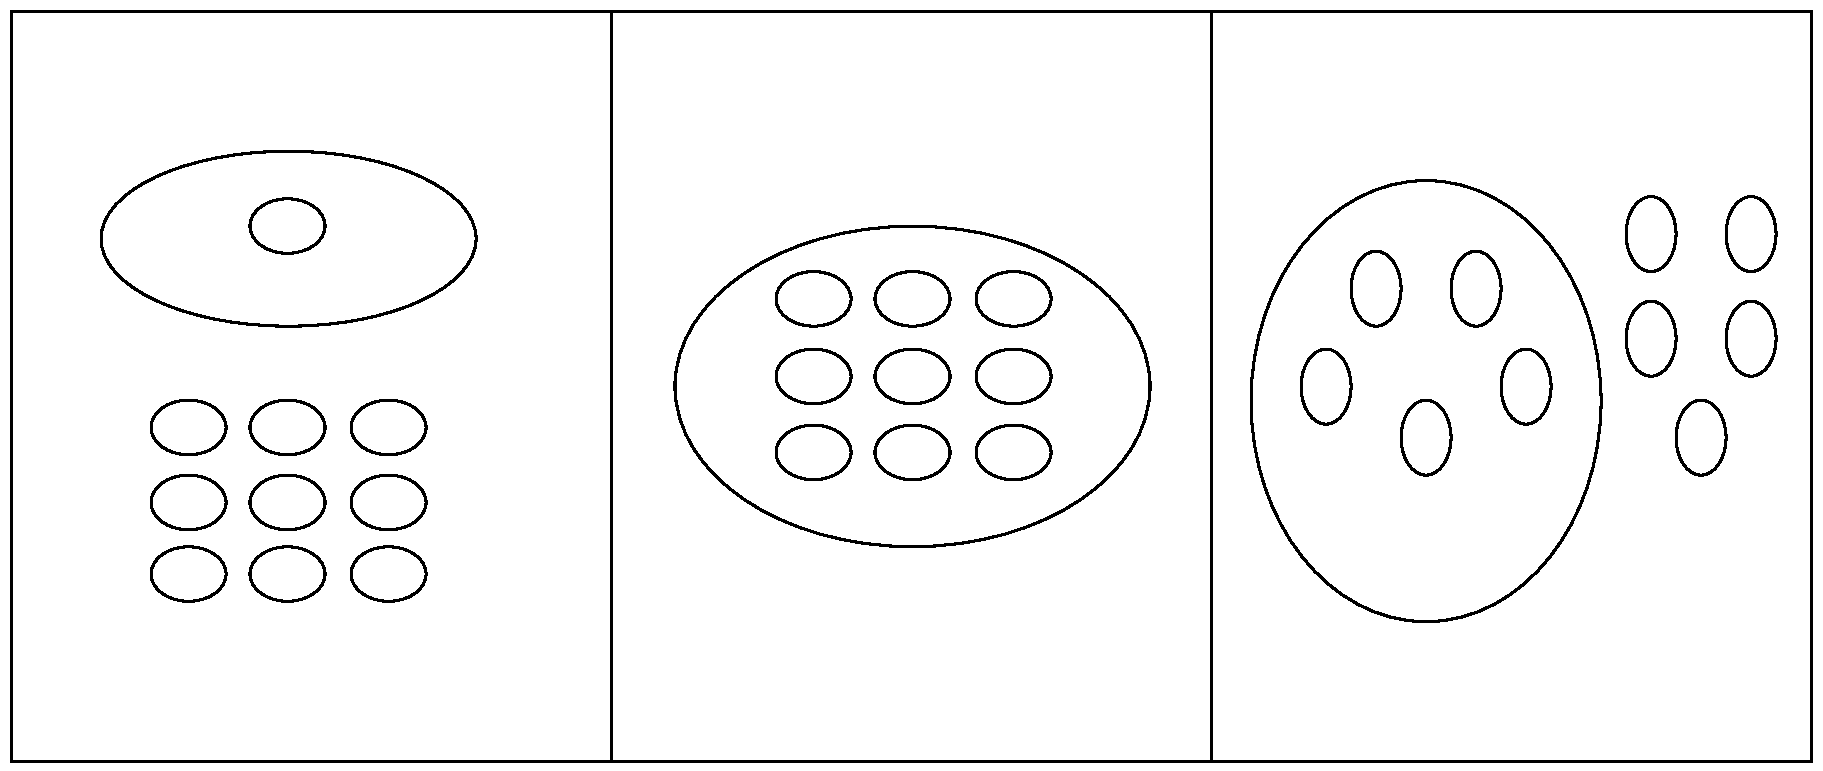
\includegraphics[scale=0.4]{Figures/fig4}
\end{center}
\caption{Classification lorsque $d=6$ avec $11$ composantes connexes}
\end{figure}
Les autres configurations sont difficiles à écarter.

\paragraph{En plus haut degré}Lorsque $d=7$ la classification est connue. Lorsque $d=8$ le problème reste ouvert.

\subsection*{Patchwork}

La technique du patchwork combinatoire permet d'établir des configurations par un procédé simple et ne dépendant pas du degré.\note{Ce serait bien de mettre un premier exemple.}

\mainmatter

\chapter{Géométrie des courbes algébriques}

\section{Lemme de \textsc{Morse}}

D'après \cite{Milnor1973}.
Par la suite, on considère $f$ à valeurs dans $\R$ définie dans un voisinage de $p\in \R^{n}$ telle que $f$ est lisse et admet un point critique en $p$. Un point critique de $f$ est non dégénéré si la forme quadratique définie par $\Delta f(p)$ est non dégénérée. L'index de $p$ pour $f$ est le nombre de $-$ qui apparaissent dans la réduction de \bsc{Gauss} de la forme quadratique précédemment évoquée.
\lemme{ 
Soit $p$ un point critique non dégénéré de $f$. Alors il existe un système de coordonnées locales $(y^{1},\ldots,y^{n})$ dans un voisinage $U$ de $p$ tel que $y^{i}(p)=0$ pour tout $i$ et aussi : \[ f= f(p) - (y^{1})^{2} -\ldots - (y^{\lambda})^{2} + (y^{\lambda+1})^{2} + \ldots + (y^{n})^{2}  \]avec $\lambda$ l'index de $f$ en $p$.
}{\textsc{Morse}}

Nous commençons par se donner un lemme préliminaire :

\lemme{
Si $f$ est lisse dans un voisinage $V$ de $0\in \R^{n}$ avec $f(0)=0$ alors \[ f(x^1,\ldots,x^n) = \sum_{i=1}^{n}x^ig_i(x^1,\ldots,x^n)\]avec des fonctions $g_i$ lisse sur $V$ et telles que\[g_i(0) = \frac{\partial f}{\partial x^{i}}(0). \]
}{}
\preuve{
Nous avons l'égalité \[f(x) = \int_{0}^{1} \frac{\dd f(tx) }{\dt}\dt = \int_{0}^{1}\sum_{i=1}^{n}\frac{\partial f}{\partial x^{i}}(tx)\cdot x^{i}\dt \]et nous définissons alors \[g_i(x) = \int_{0}^{1}\frac{\partial f}{\partial x^{i}} (tx)\dt.\]
}{}


\preuve{ 
Nous commençons par montrer que si $f$ a une telle expression alors $\lambda$ est l'index de $f$ en $p$. Supposons ainsi pour un systèmes de coordonnées $(z^{1},\ldots,z^{n})$ que \[ f(q) = f(p) - (z^{1}(q))^{2} - \ldots - (z^{\lambda}(q))^{2} + (z^{\lambda+1}(q))^{2} + \ldots + (z^{n}(\lambda))^{2}. \]Alors \[ \frac{\partial^{2} f}{\partial z^{i}\partial z^{j}}(p) = \systeme{-2 &\text{ si }i=j\leq \lambda \\ 2& \text{ si }i=j>\lambda \\0 &\text{ sinon}.}  \]

Cela montre que la matrice de $\Delta f$ selon la base $\displaystyle\der{}{z^{1}}{p},\ldots,\der{}{z^{n}}{p}$ est diagonale avec $\lambda$ fois $-2$, $(n-\lambda)$ fois $2$ sur la diagonale et dans cet ordre.

Ainsi, il existe un sous-espace de $\rT M_p$ de dimension $\lambda$ où $\Delta f$ est définie négative et un sous-espace de dimension $n-\lambda$ où $\Delta f$ est définie positive. Cela montre que $\lambda$ est l'index de $f$ en $p$.

Il nous reste à montrer qu'un tel système de coordonnées existe. Pour cela, nous commençons par supposer que $p=0$ et $f(0)=0$, par le lemme précédent nous obtenons des $g_i$ telles que \[ f(x) =\sum_{i=1}^{n} x^{i}g_i(x) .\]Comme $0$ est un point critique, $g_i(0)=0$ pour tout $i$ et donc il existe des $h_{i,j}$ telles que \[f(x) = \sum_{i,j=1}^{n}x^{i}x^{j}h_{i,j}(x). \]Nous pouvons supposer (quitte à moyenner) que $h_{i,j}=h_{j,i}$.

Pour obtenir le système de coordonnées, nous allons imiter la preuve de diagonalisation des formes quadratiques. Procédons par récurrence, supposons qu'il existe $u^{1},\ldots,u^{n}$ définies dans un voisinage $U_1$ de $0$ telles que \[f = \pm(u^{1})^{2} \pm \ldots \pm (u^{r-1})^{2} + \sum_{i,j\geq r}u^{i}u^{j}H_{i,j}(u^{1},\ldots,u^{n})\]sur $U_1$ et où la matrice  décrite par $H_{i,j}(u^{1},\ldots,u^{n})$ (de taille $(n-r+1)\times (n-r+1)$) est symétrique. Après un changement linéaire sur la dernière coordonnée, on peut faire en sorte que $H_{r,r}(0)\neq 0$. Désignons par $g(u^{1},\ldots,u^{n})$ la racine carrée de $|H_{r,r}(u^{1},\ldots,u^{n})|$. Comme $g$ est non nulle en $0$ et est lisse, il existe un voisinage $U_2\dans U_1$ de $0$ où $g$ est non nulle. On pose $v^{i}=u^{i}$ pour $i\neq r$ et \[ v^{r}(u^{1},\ldots,u^{n}) = g(u^{1},\ldots,u^{n})\left(u^r + \sum_{i>r}u^i \frac{H_{i,r}(u^{1},\ldots,u^{n})}{H_{r,r}(u^{1},\ldots,u^{n})}\right).   \]
Par le théorème d'inversion locale, $(v^{1},\ldots,v^{n})$ sera un système de coordonnées dans un voisinage $U_3\dans U_2$ de $0$. Cela complète la récurrence puisque sur $U_3$ : \[ f = \pm(v^{1})^{2} \pm \ldots \pm (v^{r})^{2} + \sum_{i,j>r}v^{i}v^{j}H_{i,j}(v^{1},\ldots,v^{n}).  \]

}{Lemme de \textsc{Morse}}


\section{Théorème des petites perturbations}

\definition{ 
Nous dirons que $\xi=(\xi_1,\xi_2,\xi_3)$ est un \emph{croisement} si $\Delta P(\xi)$ a une valeur propre strictement positive et une strictement négative.
}{}

De manière équivalente, $\xi$ est un croisement si $\xi$ est un point critique non dégénéré et d'index $1$ pour les applications : \[\fonc{\varphi_i}{\enstq{(x_0:x_1:x_2)\in \P^{2}(\R)}{x_i\neq 0}}{\R}{x}{\frac{P(x)}{x_i}\deg P} \]
\[ \tilde{P}(x_1,x_2) = P(1,x_1,x_2) \]
pour $i$ tel que $\xi_i\neq 0$.

Le lemme de \textsc{Morse} implique qu'au voisinage de $\xi$, $\R P$ est la réunion de deux droites réelles.

Réciproquement, si $\R A_1, \ldots, \R A_k$ sont non singulières, mutuellement transverse et si $3$ d'entre-elles ne se croisent jamais, alors les points critiques de $\R A_1 \cup \cdots \cup \R A_k$ sont des croisements.

Le théorème des petites perturbations s'énonce de la manière suivante :

\theoreme{ 
Soit $P$ un polynôme de degré $d$ dont les points critiques sont des croisements. Soit $Q$ un polynôme de degré $d$ dont la courbe algébrique ne passe pas par les points critiques de $P$.
 Soit $U$ un voisinage régulier de $\R P$ dans $\P^{2}(\R)$ tel que $U$ se décompose selon : \[U = U_0 \cup U_1 \]où $U_0$ est voisinage des points critiques et $U_1$ est un voisinage tubulaire de la sous-variété $\R P-U_0$ dans $\P^{2}(\R)-U_0$.

Alors il existe $X$ de degré $d$ tel que :
\begin{enumerate}
\item la courbe $\R X$ est partie de $U$ ;
\item pour chaque composante $V$ de $U_0$, il existe un homéomorphisme $h:V\to D^{1}\times D^{1}$ (avec $D^{1}$ le disque unité de dimension $1$) tel que : \[ h(\R P \cap V) = D^{1}\times \{0\} \cup  \{0\} \times D^{1},\]\[ h(\R X \cap V) = \enstq{(x,y)\in D^{1}\times D^{1}}{xy = 1/2} \; ;\]
\item $\R X -U_0$ est une section du fibré tubulaire $U_1 \to \R P-U_0$ ; 
\item $\R X \dans\enstq{(x_0:x_1:x_2)\in \P^{2}(\R)}{P(x_0,x_1,x_2)Q(x_0,x_1,x_2) \leq 0}$ ;
\item $\R X \cap \R P = \R X \cap \R Q = \R P \cap \R Q$ ;
\item si $p\in \R P\cap \R Q$ est non singulier de $Q$ et si $\R Q$ est transverse à $\R P$ en $p$ alors $\R X$ est aussi transverse à $\R P$ en $p$.
\end{enumerate}
Il existe aussi $\eps >0$ tel que pour tout $t\in ]0,\eps]$, $X=P+tQ$ convienne.
}{Petites perturbations}


\section{Théorème de \bsc{Harnack}}

\theoreme{
Pour tout entier naturel $m$ et pour tout entier $c$ vérifiant
\begin{equation}
\frac{1-(-1)^m}{2} \leq c \leq \frac{m^2-3m+4}{2} \label{HarnackIneq}
\end{equation}
il existe une courbe plane non-singulière de degré $m$ et constituée de $c$ composantes.}{\bsc{Harnack} 1876}

L'inégalité à droite de (\ref{HarnackIneq}) est l'inégalité de \bsc{Harnack}, celle de gauche découle de considérations élémentaires : une courbe de degré impair a forcément une droite projective comme composante. L'encadrement (\ref{HarnackIneq}) est donc une condition nécessaire de l'existence d'une courbe avec $c$ composantes, et le théorème affirme que cette condition est suffisante, et résout ainsi le problème de classification des courbes de degré $m$ à homéomorphisme près.

Commençons par démontrer que l'inégalité de droite de (\ref{HarnackIneq}) est optimale.

\lemme{
Pour tout entier naturel $m$, il existe une courbe de degré $m$ contenant 
$ \frac{m^2-3m+4}{2} $ composantes. Une telle courbe est appelée une M-courbe de degré $m$.} {}
\preuve{
Nous allons construire une suite de telles courbes. Le cas $m \leq 5$ a déjà été traité, on peut donc partir d'une M-courbe de degré 5, $A_5$, construite à partir de l'union de deux coniques et d'une droite $L$, perturbée en direction de l'union $B_5$ de cinq droites. 

On définit par récurrence $B_m$ pour $m > 5$ comme l'union de $m$ droites qui intersectent $\R L$ en $m$ points distincts tels que, si $m$ est pair, les points sont dans une composante arbitraire de $\R L \setminus \R B_{m-1} $, et si $m$ est impair, les points sont dans la composante de $\R L \setminus \R B_{m-1} $ qui contient $\R L \inter \R B_{m-2}$ (nous nous plaçons dans un espace projectif, il ne faut donc pas perdre de vue que le complémentaire d'un point dans une droite ne contient qu'une composante). On construit aussi $A_m$ comme une petite perturbation de $A_{m-1} \union L$ dirigée vers $B_m$. 

Pour $m>5$, supposons que $A_{m-1}$ est une M-courbe de degré $m-1$, telle que $\R A_{m-1}$ intersecte $\R L$ transversalement en $m-1$ points, placés sur une seule composante de $\R A_{m-1}$, dans le même ordre que sur $\R L$. Alors pour une certaine direction de la perturbation de $A_{m-1}$, cette composante donne $m-1$ composantes, et les $ \frac{ (m-1)^2 -3(m-1)+4 }{2} -1 = \frac{m^2-5m+6}{2} $ autres composantes ne sont que légèrement modifiées. Le nombre de composantes de $ \R A_m $ est donc : 
\[\frac{m^2-5m+6}{2} +m-1 = \frac{m^2-3m+4}{2} .\] 
$A_m$ est donc bien une M-courbe de degré $m$.

Par le théorème des petites perturbations, $\R A_m $ est transversal à $\R L$ et leur intersection est $ \R L \inter \R B_m $. Comme $ \R L \inter \R B_m $ est contenu dans une composante de $ \R L \setminus \R B_{m-1} $, il est aussi contenu dans une seule composante de $\R A_m $, et ses points apparaissent dans le même ordre sur $\R L$ que sur cette composante, ce qui termine la récurrence.\cqfd}{}

On voit aussi que l'inégalité de gauche de (\ref{HarnackIneq}) est optimale : il suffit de considérer la courbe $P(x_1,x_2,x_3) = {x_1}^m+{x_2}^m+{x_3}^m $, dont l'ensemble des zéros projectifs est vide si $m$ est pair, et est une droite projective sinon. 

Le reste de la démonstration peut se faire en construisant des courbes avec un nombre quelconque de composantes de la même manière que dans la démonstration du lemme avec des $B_m$ construits différemment. Cette démonstration est fastidieuse et n'inclut pas de nouvelles idées, nous ne la présenterons donc pas. Il existe aussi une preuve plus conceptuelle utilisant $ \R C_m $, l'espace projectif des polynômes homogènes de degré $m$.

On appelle M-courbes de \bsc{Harnack} les M-courbes pouvant être obtenues par cette méthodes (le seul degré de liberté laissé par la démonstration est, pour $m$ pair, la composante de $\R L \setminus \R B_{m-1} $ dans laquelle se trouve $\R B_m $). 

\section{Bref historique des travaux généraux après \bsc{Harnack}}

En 1891, \bsc{Hilbert} s'intéressa au problème de la classification des classes d'isotopie des courbes réelles projectives, et en particulier des M-courbes. Il remarqua que la construction de \bsc{Harnack} ne permettait pas d'obtenir tous les types d'isotopies des M-courbes, et proposa une autre construction, similaire à celle de \bsc{Harnack}, mais où les lignes sont remplacés par des coniques. Pour $ m= 6 $, la construction de \bsc{Harnack} ne donnait qu'un type d'isotopie, et celle de \bsc{Hilbert} en donnait un nouveau. \bsc{Hilbert} conjectura que ces deux types étaient les seuls possibles, mais cette conjecture fut invalidée par \bsc{Gudkov} en 1969, qui en trouva un troisième, et montra qu'il n'y avait pas plus de trois types possibles.


En 1900, \bsc{Hilbert} présenta sa célèbre liste de problèmes devant guider les mathématiques de XXème siècle, et en seizième position y figurait, notamment, la classification des types d'isotopie des courbes réelles projectives de degré 6. 

Au cours du XXème siècle, les mathématiciens cherchèrent des conditions nécessaires plus fortes que celles entraînées par le théorème de \bsc{Bezout} et l'inégalité de \bsc{Harnack}. \bsc{Ragsdale} ouvrit la voie en s'intéressant aux M-courbes de degré pair et en séparant les ovales d'une courbe en deux groupes : les ovales pairs, qui sont contenus dans un nombre pair d'autres ovales (on note $p$ leur nombre) et les ovales impairs (on note $n$ leur nombre). En étudiant les résultats des constructions de \bsc{Harnack} et de \bsc{Hilbert} pour de petits degrés, elle conjectura en 1906 des encadrements sur $p$ et $n$ pour les courbes de \bsc{Harnack} et de \bsc{Hilbert}, sur lesquels travaillèrent notamment \bsc{Petrovsky}, \bsc{Viro}, et \bsc{Itenberg}. La première nouvelle condition nécessaire portant sur toutes les M-courbes de degré pair fut le théorème de \bsc{Petrovsky} :

\theoreme{ Pour toute courbe plane projective réelle algébrique non-singulière de degré $m = 2k $ :
\[ - \frac{3}{2} k(k-1) \leq p-n \leq \frac{3}{2} k(k-1) +1.\]}{\bsc{Petrovsky} 1933-1938}

\section{L'espace des courbes algébriques réelles}

Désignons par $\R C_m$ l'ensemble des courbes algébriques réelles de degré $m$. C'est naturellement un espace projectif de dimension $m(m+3)/2$. En effet, à un polynôme, $P$, homogène de degré $m$ à trois variables, on a la représentation \[ P(x,y,z) = \sum_{i,j\geq 0\atop i+j \leq m} a_{i,j}x^{i}y^{j}z^{m-i-j}. \]

Désignons par $\R NC_m$ les courbes non-singulières. Elles forment évidemment un ouvert de $\R C_m$. De plus, localement, les courbes de $\R NC_m$ sont isotopes.

Ainsi, les différents types d'isotopies se relèvent sur les différentes composantes connexes de $\R NC_m$. Un chemin dans $\R NC_m$ donne une isotopie, dite, \emph{rigide}, entre deux courbes algébriques réelles de degré $m$.

\chapter{Point de vue complexe sur les courbes algébriques réelles}

\section{Caractéristiques topologiques complexes d'une courbe algébrique réelle}

En 1876 F. \bsc{Klein} a posé la question de type isotopique de manière plus générale. Il s'est intéressé au lien entre les points de $\R P$ et ceux de $\C P$, son analogue complexe.

Pour définir une relation de positionnement entre ces deux objets, considérons le plan projectif complexe $\P^{2}(\C)$, alors les zéros complexes de $P$ forment une sous-variété de dimension $2$ dans $\P^{2}(\C)$ que l'on appelle $\C P$.

Il s'avère que le cas complexe trivialise deux questions. La première est celle de la topologie de $\C P$, si $P$ est de degré $m$ alors $\C P$ est homéomorphe à la sphère à $(m-1)(m-2)/2$ anses. La seconde est celle du type d'isotopie du couple $(\P^{2}(\C), \C P)$, elle ne dépend que du degré de $P$.



Les points de $\R P$ se définissent comme étant les invariants par conjugaison des points de $\C P$. La conjugaison dans $\P^{2}(\C)$ étant définie par : \[\mathrm{conj}: [x:y:z]\mapsto [\barre{x}:\barre{y}:\barre{z}]. \]

La courbe $\R P$ peut, ou non, diviser en deux composantes connexes $\C P$. Dans le premier cas on dira que $\R P$ est de type I et dans le second, de type II.

Un cône projectif est homéomorphe à $\bS^{2}$. En effet, la projection stéréographique depuis un point de la conique sur une droite projective est un homéomorphisme.

La conique vide, ainsi que n'importe quelle courbe algébrique avec un ensemble vide de points réels, est de type II.  Une courbe réelle non-singulière de degré $2$ est de type 1. Ainsi, le schéma de degré $2$ $\langle 1\rangle$ est de type 1.

Pour ce qui est de l'orientation, 

\section{Théorème complexe des petites perturbations}

Considérons un premier cas élémentaire : la perturbation de droites réelles : $L_1$ et $L_2$ ces droites et $C$ le résultat. On a vu que $\C L_i$ et $\C C$ sont homéomorphes à $\bS^{2}$. Les sphères $\C L_1$ et $\C L_2$ s'intersectent à un unique point.

La version complexe du théorème des fonctions implicites montre que $\C C$ est une approximation de $\C L_1\cup \C L_2$ en dehors d'un voisinage $U_0$ de ce point d'intersection dans le sens où $\C C-U_0$ est une section du voisinage tubulaire $U_1$ de $(\C L_1 \cup \C L_2)-U_0$.

Ainsi, $\C C$ est la réunion de deux disque et d'une partie contenant un petit voisinage de $\C L_1 \cap \C L_2$.

Comme $\C C$ est homéomorphe à $\bS^{2}$ et que le complémentaire de deux disques disjoints plongés dans $\bS^{2}$ est homéomorphe à un anneau, la troisième partie de $\C C$ en est un. Les disques sont les complémentaires d'un voisinage de $\C L_1\cap \C L_2$ respectivement dans $\C L_1$ et $\C L_2$, légèrement perturbés dans $\P^{2}(\C)$ et l'anneau connecte ces deux disques à travers le voisinage $U_0$ de $\C L_1\cap \C L_2$.


Jusqu'ici, il n'y a pas d'importance quant à la nature réelle des courbes en jeu.
Pour se ramener au cas réel, il faut décrire la position des parties réelles des courbes dans leurs complexifiées and l'action de conjugaison.

Le montage complexe précédent est invariant par conjugaison, donc l'intersection de $\C L_1$ et $\C L_2$ est réelle et son voisinage $U_0$ peut être choisi comme invariant par l'action de conjugaison.
Donc $\C C$ se représente comme la réunion de deux demi-disques et d'un demi-anneau : les demi-disques approchent les moitiés de $\C L_1$ et $\C L_2$ et un moitié de l'anneau est contenue dans $U_0$.

Il reste à spécifier quels sont les demi-disques connectés par un demi-anneau.


Dans le cas général, commençons par considérer l'objet complexe tel quel. Considérons une surface algébrique qui n'a que des points doubles non dégénérés. Près d'un tel point, on reconnait la réunion de deux droites s'intersectant en ce point. Cela signifie qu'il existe un voisinage $U$ de ce point dans $\P^{2}(\C)$ et un difféomorphisme qui envoie $U$ dans $\C^{2}$ en associant l'intersection de $U$ et la courbe à l'union de deux droites complexes qui s'intersectent en $0$. Cela vient de la version complexe du lemme de \bsc{Morse}. Encore par ce lemme, près d'un point double, le théorème des petites perturbations classique applique une petite perturbation à la réunion des deux droites : la réunion de deux disques transverses est remplacée par un anneau.


Par exemple, prenons la réunion de $m$ droites projectives dont $3$ n'ont pas de point en commun. Ses points complexes sont la réunion de $m$ copies de $\bS^{2}$ telles que deux ont exactement un point en commun. Une perturbation peut être pensée comme le découpage dans chacune des sphères de $m-1$ disques et au recollage de $m(m-1)/2$ tubes connectant les frontières des disques découpés. Le résultat est orientable (en tant que variété complexe). On obtient alors une sphère avec $(m-2)(m-1)/2$ anses.




\printbibliography
\end{document}
